\section{Introduzione}

\subsection{Obiettivo}
L'obiettivo di questa tesi riguarda lo studio teorico e l'implementazione pratica di approcci di controllo centralizzato ad un manipolatore a cinematica parallela, avente 4 gradi di libertà, con l'obiettivo di andare a trovare la tecnica migliore. In primis verrà eseguita una modellazione meccanica teorica, successivamente mediante un'attività sperimentale che comprende l'implementazione degli schemi di controllo analizzati e la generazione di traiettorie bidimensionali e tridimensionali, si andranno ad analizzare i risultati ottenuti.
\subsection{Stato dell'arte}
Il lavoro di tesi è stato svolto in collaborazione con il laboratorio di meccatronica dell'università degli studi di Bergamo. Alla base di questa tesi vi è il manipolatore PKM (\textit{parallel kinematic manipulator}) costruito nel 2013. Un manipolatore parallelo è un sistema meccanico che utilizza "catene" seriali per supportare un \textit{end-effector}, ogni catena solitamente è corta, semplice e di conseguenza può essere rigida rispetto a movimenti non voluti rispetto ad un manipolatore seriali. La movimentazione e la flessibilità di un \textit{joint} è vincolata dall'effetto delle altre catene, questo rende il manipolatore rigido rispetto alle sue componenti. 
\par In particolare, nel nostro caso il manipolatore è composto da cinque giunti rotoidali, quattro link, di cui due motorizzati e all'estermità è connessa una vite che consente traslazione e rotazione nell'asse Z, in questa configurazione il robot arriva ad avere 4 gradi di libertà.
\begin{figure}[ht]
	\begin{center}
		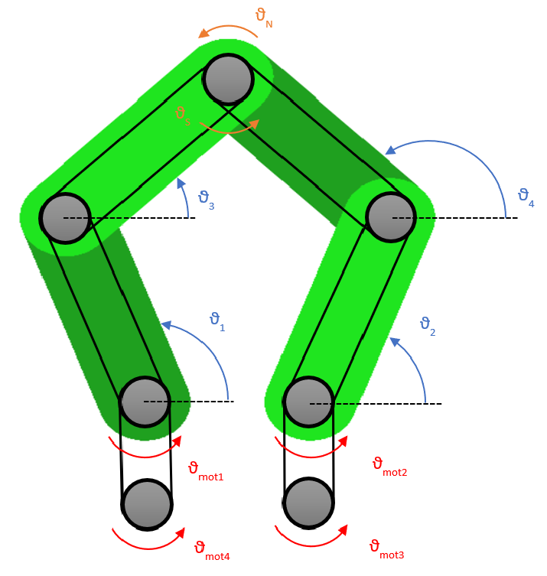
\includegraphics[scale=0.7]{Immagini/Robot1.png}
		\caption{Robot PKM 
		\label{fig:PKM}}
	\end{center}
\end{figure}
Escludendo l'introduzione, il lavoro di tesi sarà articolato in sette capitoli: nel secondo capitolo verrà presentata l'analisi cinematica del manipolatore, in particolare verranno analizzate sia cinematica diretta che inversa, nel terzo capitolo si parlerà di dinamica, nel quarto tratteremo i punti di singolarità e manipolabilità del robot; il quinto capitolo mostrerà la modellazione dell'\textit{end-effector}, nel nostro caso la vite; il sesto capitolo andrà a presentare tutte le tecnologie implementate a livello pratico, nel settimo capitolo verrà presentato il sistema reale, includendo la struttura, le modalità di comunicazione, il software implementato, il sistema di controllo, l'interfaccia grafica ed i problemi riscontrati con le relative soluzioni. Infine, nell'ottavo capitolo, verranno esposte le conclusioni, e gli sviluppi futuri.
\subsection{Ambiti applicativi}
Grazie alle loro caratteristiche, i manipolatori a cinematica parallela vengono utilizzati in diversi ambiti, di seguito è riportato solo qualche esempio:
\begin{itemize}
	\item Simulatori di volo
	\item Simulatori di guida
	\item Allineamento e posizionamento della fibra ottica
	\item Ambito medicale
	\item Assemblamento \textit{PCB}
	\item Operazioni di \textit{pick $\&$ place}
\end{itemize}

\subsection{Software modellazione teorica}
Per la modellazione teorica del manipolatore, abbiamo bisogno di utilizzare strumenti software specifici; in particolare verranno utilizzati Matlab e Adams, il primo ci consentirà di realizzare un modello software del manipolatore, il secondo, sempre a partire da un modello ci servirà a validare i dati ottenuti dal primo in modo da verificare la loro correttezza.
\subsubsection{Matlab}
Matlab, abbreviazione di \textit{Matrix Laboratory}, è una piattaforma di calcolo ottimizzata nella risoluzione di problemi tecnici. 
Matlab è un linguaggio ad alte prestazione per la computazione tecnica, comprende: computazione, visualizzazione e programmazione in un ambiente di facile utilizzo dove i problemi e le soluzioni vengono espressi mediante una notazione matematica, gli utilizzi tipici riguardano: matematica, sviluppo di algoritmi, modellazione, simulazione, prototipazione, analisi dei dati, intelligenza artificiale, verifiche di computazione. La base di matlab è un vettore che non ha bisogno di dimensioni, in questo modo permette la risoluzione di molti problemi di computazione, specialmente quelli in formulazione vettoriale e matriciale velocemente, senza dover ricorrere all'utilizzo di linguaggi come il C. Matlab inoltre possiede delle \textit{toolbox} ovvero moduli aggiuntivi che permettono di specializzarsi in un campo, in particolare sono insieme di funzioni MATLAB che estendono l'ambiente, permettendogli di risolvere particolari classi di problemi, esempi di moduli sono reti neurali, processamento di segnali, sistemi di controllo.
\par Nel nostro caso abbiamo definito il modello teorico del robot, abbiamo poi calcolato cinematica, dinamica e punti di singolarità, nei capitoli successivi verranno mostrate le operazioni fatte. 
\subsubsection{Adams}
Adams è un software utilizzato nel campo della dinamica \textit{multibody}, in particolare nell'analisi dei modelli, infatti dopo che è stato progettato un modello può essere importato in adams ed è possibile fare analisi, simulazioni e validazioni, andando quindi a simulare la fisica del mondo reale. Adams è anche ottimizzato per problemi di grandi dimensioni.
\par Il software ha una GUI completa, infatti consente anche di disegnare direttamente il modello nello spazio tridimensionale o di importare file come STEP e IGS. I \textit{joint} possono essere aggiunti tra due corpi per vincolare il loro movimento, inoltre al sistema possono essere passati input come velocità, forze e condizioni iniziali. Adams simula il comportamento del sistema al variare del tempo, consente anche l'animazione e la computazione di proprietà come le forze, le inerzie e le accelerazioni, è anche possibile nel sistema includere elementi complessi dinamicamente come per esempio molle, corpo flessibili, contatto tra corpi.
É inoltre possibile esportare tutti i dati in formato tabellare per fare analisi successive. 
\par Per quanto riguarda il nostro caso, abbiamo utilizzato Adams per modellare il robot, assegnargli le coppie e confrontare i valori della cinematica e dinamica con quelli ottenuti da Matlab, nei capitoli successivi verrà presentato un confronto tra questi dati.